\section{Resultados e Discussões}

Cada tempo de reação foi medido uma única vez, de modo que não é possível estimar sua incerteza pela dispersão de medidas repetidas. A resolução do cronômetro ($0{,}01\un{s}$) é muito menor que o tempo de reação do operador e a incerteza na identificação visual do aparecimento da cor azul, estimadas em algumas décimas de segundo. Por isso, as incertezas dos parâmetros ajustados foram obtidas pela dispersão dos pontos em torno das retas (Seção~\ref{sec:mmq}).

\subsection{Influência da concentração na velocidade da reação}

Pela Equação~\eqref{eq:diluicao}, a concentração de \ce{KIO3} após a mistura para a amostra A, por exemplo, é
\[
[\ce{KIO3}]_A=\frac{(2{,}000\times10^{-2})\cdot5{,}00}{100}=1{,}000\times10^{-3}\un{mol/L},
\]
e, analogamente, para as demais amostras. A concentração de \ce{NaHSO3} após a mistura é $8{,}19\times10^{-4}\un{mol/L}$ em todas elas. O tempo da amostra A, $1\un{min}\,26{,}72\un{s}$, corresponde a $86{,}72\un{s}$, e seu inverso é $1/86{,}72=1{,}153\times10^{-2}\un{s^{-1}}$. Os resultados estão reunidos na Tabela~\ref{tab:resultadosA}.

\begin{table}[H]
\centering
\caption{Composição das amostras, tempo de reação, tempo inverso e concentração molar após a mistura ($V_f=100\un{mL}$).}
\label{tab:resultadosA}
{\small\setlength{\tabcolsep}{4pt}
\begin{tabular}{ccccccc}
\toprule
\multirow{2}{*}{Amostra} & Solução 1 & Solução 2 & Tempo de & Tempo inverso & \multicolumn{2}{c}{Concentração ($10^{-3}\un{mol/L}$)} \\
\cmidrule(lr){6-7}
 & (mL) & (mL) & reação (s) & ($10^{-2}\un{s^{-1}}$) & \ce{KIO3} & \ce{NaHSO3} \\
\midrule
A & 5,00 & 10,00 & 86,72 & 1,153 & 1,000 & 0,819 \\
B & 10,00 & 10,00 & 42,42 & 2,357 & 2,000 & 0,819 \\
C & 15,00 & 10,00 & 29,64 & 3,374 & 3,000 & 0,819 \\
D & 20,00 & 10,00 & 21,38 & 4,677 & 4,000 & 0,819 \\
E & 25,00 & 10,00 & 18,05 & 5,540 & 5,000 & 0,819 \\
Desconhecida & -- & 10,00 & 44,61 & 2,242 & $1{,}94\pm0{,}12$ & 0,819 \\
\bottomrule
\end{tabular}}
\fonte{Elaborada pelos autores.}
\end{table}

Observa-se que o tempo de reação diminui à medida que a concentração de iodato aumenta: dobrando-se a concentração de A para B, o tempo cai praticamente à metade ($86{,}72\un{s}\to42{,}42\un{s}$), e, ao quintuplicá-la (de A para E), o tempo fica cerca de $4{,}8$ vezes menor. Isso está de acordo com a teoria das colisões, já que uma maior concentração de \ce{IO3-} aumenta o número de colisões por unidade de tempo e, portanto, a velocidade com que o hidrogenossulfito é consumido.

\subsubsection{Curva de calibração}

A Figura~\ref{fig:calibracao} mostra o tempo inverso em função da concentração de \ce{KIO3} após a mistura. Ajustando uma reta $1/t=a+b\,[\ce{KIO3}]$ aos cinco pontos pelo método dos mínimos quadrados, obteve-se
\begin{gather*}
b=(11{,}1\pm0{,}4)\un{L\,mol^{-1}\,s^{-1}},\\
a=(0{,}9\pm1{,}2)\times10^{-3}\un{s^{-1}},\\
s_r=1{,}13\times10^{-3}\un{s^{-1}},\qquad r=0{,}9985.
\end{gather*}
O coeficiente de correlação próximo de 1 indica que os pontos estão bem alinhados, e o coeficiente linear é compatível com zero dentro de sua incerteza. Isso mostra que $1/t$ é, dentro do erro experimental, diretamente proporcional à concentração de iodato, como esperado para uma reação de primeira ordem em relação ao \ce{IO3-} (Equação~\ref{eq:ordem} com $n=1$). Os resíduos ($-0{,}5$; $0{,}5$; $-0{,}5$; $1{,}5$ e $-1{,}0\times10^{-3}\un{s^{-1}}$) não apresentam tendência sistemática, sendo o maior deles o da amostra D.

\begin{figure}[H]
\centering
\caption{Curva de calibração: tempo inverso em função da concentração de \ce{KIO3} após a mistura. O ponto vazado indica a amostra desconhecida, interpolada na reta.}
\label{fig:calibracao}
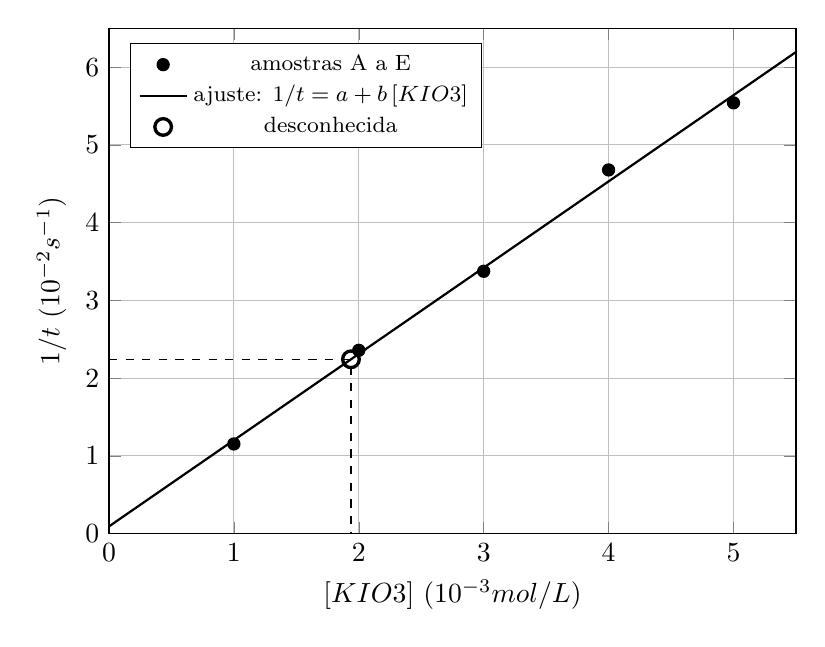
\begin{tikzpicture}
\begin{axis}[
  width=0.85\textwidth, height=8cm,
  xlabel={$[\ce{KIO3}]$ ($10^{-3}\un{mol/L}$)}, ylabel={$1/t$ ($10^{-2}\un{s^{-1}}$)},
  xmin=0, xmax=5.5, ymin=0, ymax=6.5,
  grid=both, legend pos=north west, legend style={font=\footnotesize},
]
\addplot[only marks, mark=*, mark size=2.2pt] coordinates {
(1.000,1.1531) (2.000,2.3574) (3.000,3.3738) (4.000,4.6773) (5.000,5.5402)
};
\addlegendentry{amostras A a E}
\addplot[domain=0:5.5, samples=2, thick] {0.09217+1.10939*x};
\addlegendentry{ajuste: $1/t=a+b\,[\ce{KIO3}]$}
\addplot[only marks, mark=o, mark size=3pt, very thick] coordinates {(1.9375,2.2416)};
\addlegendentry{desconhecida}
\addplot[dashed] coordinates {(0,2.2416) (1.9375,2.2416) (1.9375,0)};
\end{axis}
\end{tikzpicture}
\fonte{Elaborada pelos autores.}
\end{figure}

\subsubsection{Concentração da solução desconhecida}

Para a amostra desconhecida, o tempo de reação foi $44{,}61\un{s}$, ou seja, $1/t=2{,}242\times10^{-2}\un{s^{-1}}$. Interpolando na curva de calibração,
\[
[\ce{KIO3}]_x=\frac{1/t-a}{b}=\frac{2{,}242\times10^{-2}-9{,}2\times10^{-4}}{11{,}09}=1{,}94\times10^{-3}\un{mol/L},
\]
e, pela Equação~\eqref{eq:ucal}, com $N=5$, $\overline{1/t}=3{,}420\times10^{-2}\un{s^{-1}}$ e $S_{xx}=1{,}0\times10^{-5}\un{mol^2/L^2}$,
\begin{gather*}
u([\ce{KIO3}]_x)=\frac{1{,}13\times10^{-3}}{11{,}09}\sqrt{1+\frac{1}{5}+\frac{(2{,}242\times10^{-2}-3{,}420\times10^{-2})^2}{11{,}09^2\cdot1{,}0\times10^{-5}}},\\
u([\ce{KIO3}]_x)=0{,}12\times10^{-3}\un{mol/L}.
\end{gather*}
Assim, a concentração de iodato na mistura da amostra desconhecida é
\[
[\ce{KIO3}]_x=(1{,}94\pm0{,}12)\times10^{-3}\un{mol/L}.
\]
Caso se force a reta a passar pela origem (isto é, $1/t=b_0[\ce{KIO3}]$, com $b_0=(11{,}35\pm0{,}14)\un{L\,mol^{-1}\,s^{-1}}$), obtém-se $1{,}98\times10^{-3}\un{mol/L}$, valor compatível com o anterior. O resultado situa-se entre as amostras A e B, como esperado, já que o tempo da desconhecida ($44{,}61\un{s}$) ficou entre os delas e muito próximo do da amostra B ($42{,}42\un{s}$). Ele equivale à concentração que seria obtida com cerca de $9{,}7\un{mL}$ da Solução 1 ($[\ce{KIO3}]_x\cdot V_f/c_1$). Se a solução desconhecida foi utilizada em um volume $V_x$ no lugar da Solução 1, sua concentração original é dada por $c_x=[\ce{KIO3}]_x\,V_f/V_x$.

\subsubsection{Ordem da reação em relação ao iodato}

Para verificar a hipótese de primeira ordem, ajustou-se uma reta ao gráfico de $\ln(1/t)$ em função de $\ln[\ce{KIO3}]$, conforme a Equação~\eqref{eq:ordem}, como mostra a Figura~\ref{fig:ordem}. O coeficiente angular obtido foi
\[
n=0{,}98\pm0{,}02,\qquad r=0{,}9993,
\]
compatível com $n=1$. Portanto, nas condições do experimento, a velocidade da reação é diretamente proporcional à concentração de iodato: ao dobrar $[\ce{IO3-}]$, a velocidade dobra e o tempo de reação cai à metade.

\begin{figure}[H]
\centering
\caption{Gráfico log-log do tempo inverso em função da concentração de \ce{KIO3}. O coeficiente angular corresponde à ordem da reação em relação ao iodato.}
\label{fig:ordem}
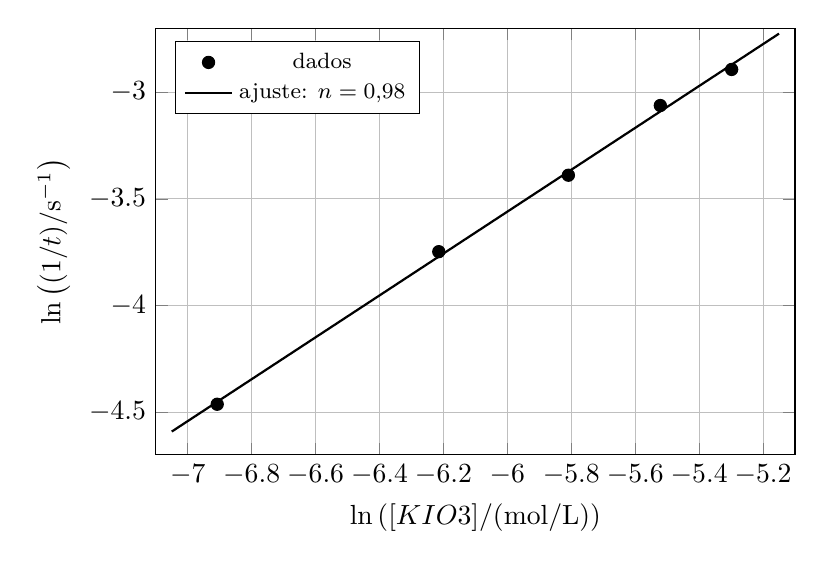
\begin{tikzpicture}
\begin{axis}[
  width=0.8\textwidth, height=7cm,
  xlabel={$\ln\left([\ce{KIO3}]/(\mathrm{mol/L})\right)$}, ylabel={$\ln\left((1/t)/\mathrm{s^{-1}}\right)$},
  xmin=-7.1, xmax=-5.1, ymin=-4.7, ymax=-2.7,
  grid=both, legend pos=north west, legend style={font=\footnotesize},
]
\addplot[only marks, mark=*, mark size=2.2pt] coordinates {
(-6.9078,-4.4627) (-6.2146,-3.7475) (-5.8091,-3.3891) (-5.5215,-3.0624) (-5.2983,-2.8932)
};
\addlegendentry{dados}
\addplot[domain=-7.05:-5.15, samples=2, thick] {2.33109+0.98182*x};
\addlegendentry{ajuste: $n=0{,}98$}
\end{axis}
\end{tikzpicture}
\fonte{Elaborada pelos autores.}
\end{figure}

\subsection{Influência da temperatura na velocidade da reação}

A Tabela~\ref{tab:temperatura} apresenta os tempos de reação obtidos com a composição da amostra C ($[\ce{KIO3}]=3{,}000\times10^{-3}\un{mol/L}$ e $[\ce{NaHSO3}]=8{,}19\times10^{-4}\un{mol/L}$) em três temperaturas. O ensaio à temperatura ambiente ($25\un{^\circ C}$) é o próprio ensaio da amostra C da parte A. Para o ensaio a frio, cuja temperatura ficou entre $4$ e $6\un{^\circ C}$, adotou-se $T=(5\pm1)\un{^\circ C}$.

\begin{table}[H]
\centering
\caption{Temperaturas das amostras, tempo de reação e tempo recíproco.}
\label{tab:temperatura}
{\small\setlength{\tabcolsep}{4pt}
\begin{tabular}{cccccc}
\toprule
Amostra & Temperatura ($^\circ$C) & $T$ (K) & $t$ (s) & $1/t$ ($10^{-2}\un{s^{-1}}$) & $\ln(1/t)$ \\
\midrule
T1 (ambiente) & 25 & 298,15 & 29,64 & 3,374 & $-3{,}389$ \\
T2 ($15\un{^\circ C}$) & 15 & 288,15 & 42,47 & 2,355 & $-3{,}749$ \\
T3 ($4$ a $6\un{^\circ C}$) & $5\pm1$ & 278,15 & 59,59 & 1,678 & $-4{,}087$ \\
\bottomrule
\end{tabular}}
\fonte{Elaborada pelos autores.}
\end{table}

Com a diminuição da temperatura, o tempo de reação aumenta, isto é, a velocidade diminui. Comparando com a amostra C à temperatura ambiente, a velocidade a $15\un{^\circ C}$ é $29{,}64/42{,}47=0{,}70$ vez a velocidade a $25\un{^\circ C}$ e, a $5\un{^\circ C}$, cerca de $29{,}64/59{,}59=0{,}50$ vez, ou seja, a reação ficou aproximadamente duas vezes mais lenta com um resfriamento de $20\un{^\circ C}$. Isso confirma que a temperatura é um fator determinante da velocidade: em temperatura mais baixa, a energia cinética média das moléculas é menor, as colisões são menos frequentes e, principalmente, uma fração menor delas tem energia suficiente para superar a energia de ativação.

\subsubsection{Energia de ativação}

A Figura~\ref{fig:arrhenius} mostra o gráfico de Arrhenius, $\ln(1/t)$ em função de $1/T$. Os três pontos estão bem alinhados ($r=-0{,}9993$), e o ajuste linear fornece o coeficiente angular
\[
-\frac{E_a}{R}=(-2{,}89\pm0{,}11)\times10^{3}\un{K},
\]
de onde
\[
E_a=8{,}314\cdot2{,}89\times10^{3}=(24{,}1\pm0{,}9)\un{kJ/mol}.
\]
Aplicando a Equação~\eqref{eq:Ea2} a cada par de temperaturas, obtém-se $E_a=25{,}7\un{kJ/mol}$ entre $25$ e $15\un{^\circ C}$ e $E_a=22{,}6\un{kJ/mol}$ entre $15$ e $5\un{^\circ C}$, valores próximos ao do ajuste. Considerando os extremos da faixa de temperatura do ensaio a frio ($4$ e $6\un{^\circ C}$), o ajuste fornece $E_a$ entre $22{,}8$ e $25{,}4\un{kJ/mol}$, de modo que a incerteza na temperatura desse ensaio tem efeito comparável ao da dispersão dos pontos.

\begin{figure}[H]
\centering
\caption{Gráfico de Arrhenius: logaritmo do tempo recíproco em função do inverso da temperatura absoluta.}
\label{fig:arrhenius}
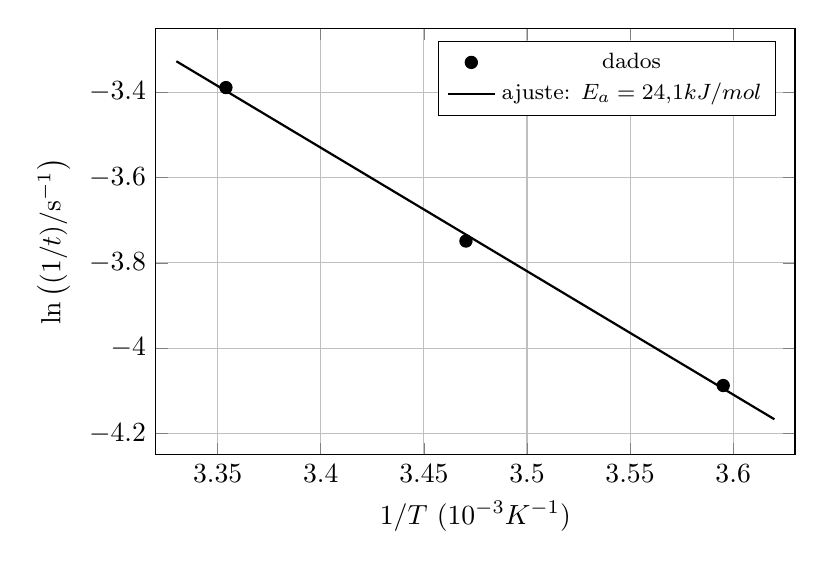
\begin{tikzpicture}
\begin{axis}[
  width=0.8\textwidth, height=7cm,
  xlabel={$1/T$ ($10^{-3}\un{K^{-1}}$)}, ylabel={$\ln\left((1/t)/\mathrm{s^{-1}}\right)$},
  xmin=3.32, xmax=3.63, ymin=-4.25, ymax=-3.25,
  xtick={3.35,3.40,3.45,3.50,3.55,3.60},
  grid=both, legend pos=north east, legend style={font=\footnotesize},
  xticklabel style={/pgf/number format/fixed, /pgf/number format/precision=2},
]
\addplot[only marks, mark=*, mark size=2.2pt] coordinates {
(3.35402,-3.38912) (3.47041,-3.74880) (3.59518,-4.08749)
};
\addlegendentry{dados}
\addplot[domain=3.33:3.62, samples=2, thick] {6.30829-2.89361*x};
\addlegendentry{ajuste: $E_a=24{,}1\un{kJ/mol}$}
\end{axis}
\end{tikzpicture}
\fonte{Elaborada pelos autores.}
\end{figure}

A regra empírica citada na apostila, segundo a qual a velocidade dobra a cada aumento de $10\un{^\circ C}$, corresponde, próximo da temperatura ambiente, a uma energia de ativação de cerca de $50\un{kJ/mol}$. No experimento, a velocidade aumentou por um fator de aproximadamente $1{,}4$ a cada $10\un{^\circ C}$, o que corresponde ao valor menor de $E_a$ obtido. Parte dessa diferença pode ser atribuída ao procedimento: a mistura foi feita fora do banho de gelo e a reação se desenvolveu durante $40$ a $60\un{s}$ em contato com o ambiente a $25\un{^\circ C}$, de modo que a temperatura média da solução durante a reação deve ter sido maior que a registrada no momento da mistura. Isso torna os ensaios a frio mais rápidos do que seriam a temperatura constante e leva a subestimar $E_a$. Além disso, a regra do fator 2 é apenas uma aproximação, válida para muitas reações, mas não para todas.

\subsection{Fontes de erro}

As principais fontes de erro do experimento foram:
\begin{itemize}
    \item \textbf{identificação do ponto final}: o aparecimento da cor azul é avaliado visualmente, e diferentes observadores podem considerar instantes ligeiramente distintos;
    \item \textbf{cronometragem}: o tempo de reação do operador ao iniciar e parar o cronômetro, além do tempo gasto para verter a solução 2 sobre a solução 1, afetam proporcionalmente mais os ensaios mais rápidos (amostras D e E);
    \item \textbf{medidas de volume}: erros de leitura nas buretas e no ajuste do menisco nos balões volumétricos alteram as concentrações das amostras;
    \item \textbf{temperatura}: nos ensaios a frio, a temperatura da solução variou durante a reação, e a do terceiro ensaio só é conhecida dentro da faixa de $4$ a $6\un{^\circ C}$; na parte A, pequenas variações da temperatura ambiente entre ensaios também afetam os tempos;
    \item \textbf{medidas únicas}: cada tempo foi medido uma só vez, o que impede estimar diretamente sua incerteza e torna os resultados sensíveis a erros pontuais, como o da amostra D, que apresentou o maior resíduo na curva de calibração;
    \item \textbf{contaminação}: resíduos de ensaios anteriores nos béqueres, caso a lavagem não seja completa, podem alterar as concentrações.
\end{itemize}
